\documentclass[a4paper]{article}
\usepackage{lmodern}
\usepackage{amssymb,amsmath}
\usepackage{ifxetex,ifluatex}
\usepackage{fixltx2e} % provides \textsubscript
\ifnum 0\ifxetex 1\fi\ifluatex 1\fi=0 % if pdftex
  \usepackage[T1]{fontenc}
  \usepackage[utf8]{inputenc}
\else % if luatex or xelatex
  \ifxetex
    \usepackage{mathspec}
  \else
    \usepackage{fontspec}
  \fi
  \defaultfontfeatures{Ligatures=TeX,Scale=MatchLowercase}
\fi
% use upquote if available, for straight quotes in verbatim environments
\IfFileExists{upquote.sty}{\usepackage{upquote}}{}
% use microtype if available
\IfFileExists{microtype.sty}{%
\usepackage{microtype}
\UseMicrotypeSet[protrusion]{basicmath} % disable protrusion for tt fonts
}{}
\usepackage{hyperref}
\hypersetup{unicode=true,
            pdftitle={Estudos de caso},
            pdfborder={0 0 0},
            breaklinks=true}
\urlstyle{same}  % don't use monospace font for urls
\usepackage{graphicx,grffile}
\makeatletter
\def\maxwidth{\ifdim\Gin@nat@width>\linewidth\linewidth\else\Gin@nat@width\fi}
\def\maxheight{\ifdim\Gin@nat@height>\textheight\textheight\else\Gin@nat@height\fi}
\makeatother
% Scale images if necessary, so that they will not overflow the page
% margins by default, and it is still possible to overwrite the defaults
% using explicit options in \includegraphics[width, height, ...]{}
\setkeys{Gin}{width=\maxwidth,height=\maxheight,keepaspectratio}
\IfFileExists{parskip.sty}{%
\usepackage{parskip}
}{% else
\setlength{\parindent}{0pt}
\setlength{\parskip}{6pt plus 2pt minus 1pt}
}
\setlength{\emergencystretch}{3em}  % prevent overfull lines
\providecommand{\tightlist}{%
  \setlength{\itemsep}{0pt}\setlength{\parskip}{0pt}}
\setcounter{secnumdepth}{5}
% Redefines (sub)paragraphs to behave more like sections
\ifx\paragraph\undefined\else
\let\oldparagraph\paragraph
\renewcommand{\paragraph}[1]{\oldparagraph{#1}\mbox{}}
\fi
\ifx\subparagraph\undefined\else
\let\oldsubparagraph\subparagraph
\renewcommand{\subparagraph}[1]{\oldsubparagraph{#1}\mbox{}}
\fi

%%% Use protect on footnotes to avoid problems with footnotes in titles
\let\rmarkdownfootnote\footnote%
\def\footnote{\protect\rmarkdownfootnote}

%%% Change title format to be more compact
\usepackage{titling}

% Create subtitle command for use in maketitle
\providecommand{\subtitle}[1]{
  \posttitle{
    \begin{center}\large#1\end{center}
    }
}

\setlength{\droptitle}{-2em}

  \title{Estudos de caso}
    \pretitle{\vspace{\droptitle}\centering\huge}
  \posttitle{\par}
  \subtitle{Aplicações na Engenharia de Avaliações}
  \author{}
    \preauthor{}\postauthor{}
      \predate{\centering\large\emph}
  \postdate{\par}
    \date{11/08/2019}

\usepackage[brazil]{babel}
\usepackage{graphicx}
\usepackage{float}
\usepackage{subfig}
\usepackage{caption}
\newcommand{\pkg}[1]{{\normalfont\fontseries{b}\selectfont #1}}
\let\proglang=\textsf
\let\code=\texttt

\begin{document}
\maketitle

\hypertarget{estudos-de-caso}{%
\section{Estudos de Caso}\label{estudos-de-caso}}

Para os estudos de caso foram utilizados os dados disponíveis em
HOCHHEIM (\protect\hyperlink{ref-hochheim}{2015}).

\hypertarget{duas-dimensoes}{%
\subsection{Duas dimensões}\label{duas-dimensoes}}

Assim como na regressão linear, é mais fácil aa compreensão da regressão
quantílica através de exemplos em duas dimensões, e depois generalizar
para \(n\) dimensões.

Seja primeiramente o caso de dados heteroscedásticos. A figura
\ref{fig:qr1} ilustra a aplicação da regressão quantílica e da regressão
linear para este caso. Na figura \ref{fig:qr1}, a reta vermelha é a reta
de regressão linear entre as variáveis. A área sombreada em cinza é o
intervalo de confiança para a regressão linear @80\%. As retas azuis são
as retas de regressão quantílica para os quantis 0,1; 0,2; 0,3; 0,4;
0,5; 0,6; 0,7; 0,8 e 0,9.

A regressão quantílica neste caso pode ser usada para demonstrar a não
validade dos intervalos de confiança (IC) e predição (IP) para a
regressão linear para este tipo de dados: como a variância da população
não é constante, mas aumenta com o aumento da área, as retas da
regressão quantílica se abrem. Como os intervalos de confiança e
predição na inferência clássica são calculados considerando-se que a
variância da população é constante, este efeito não se observa no
formato do IC.

\begin{figure}[H]

{\centering 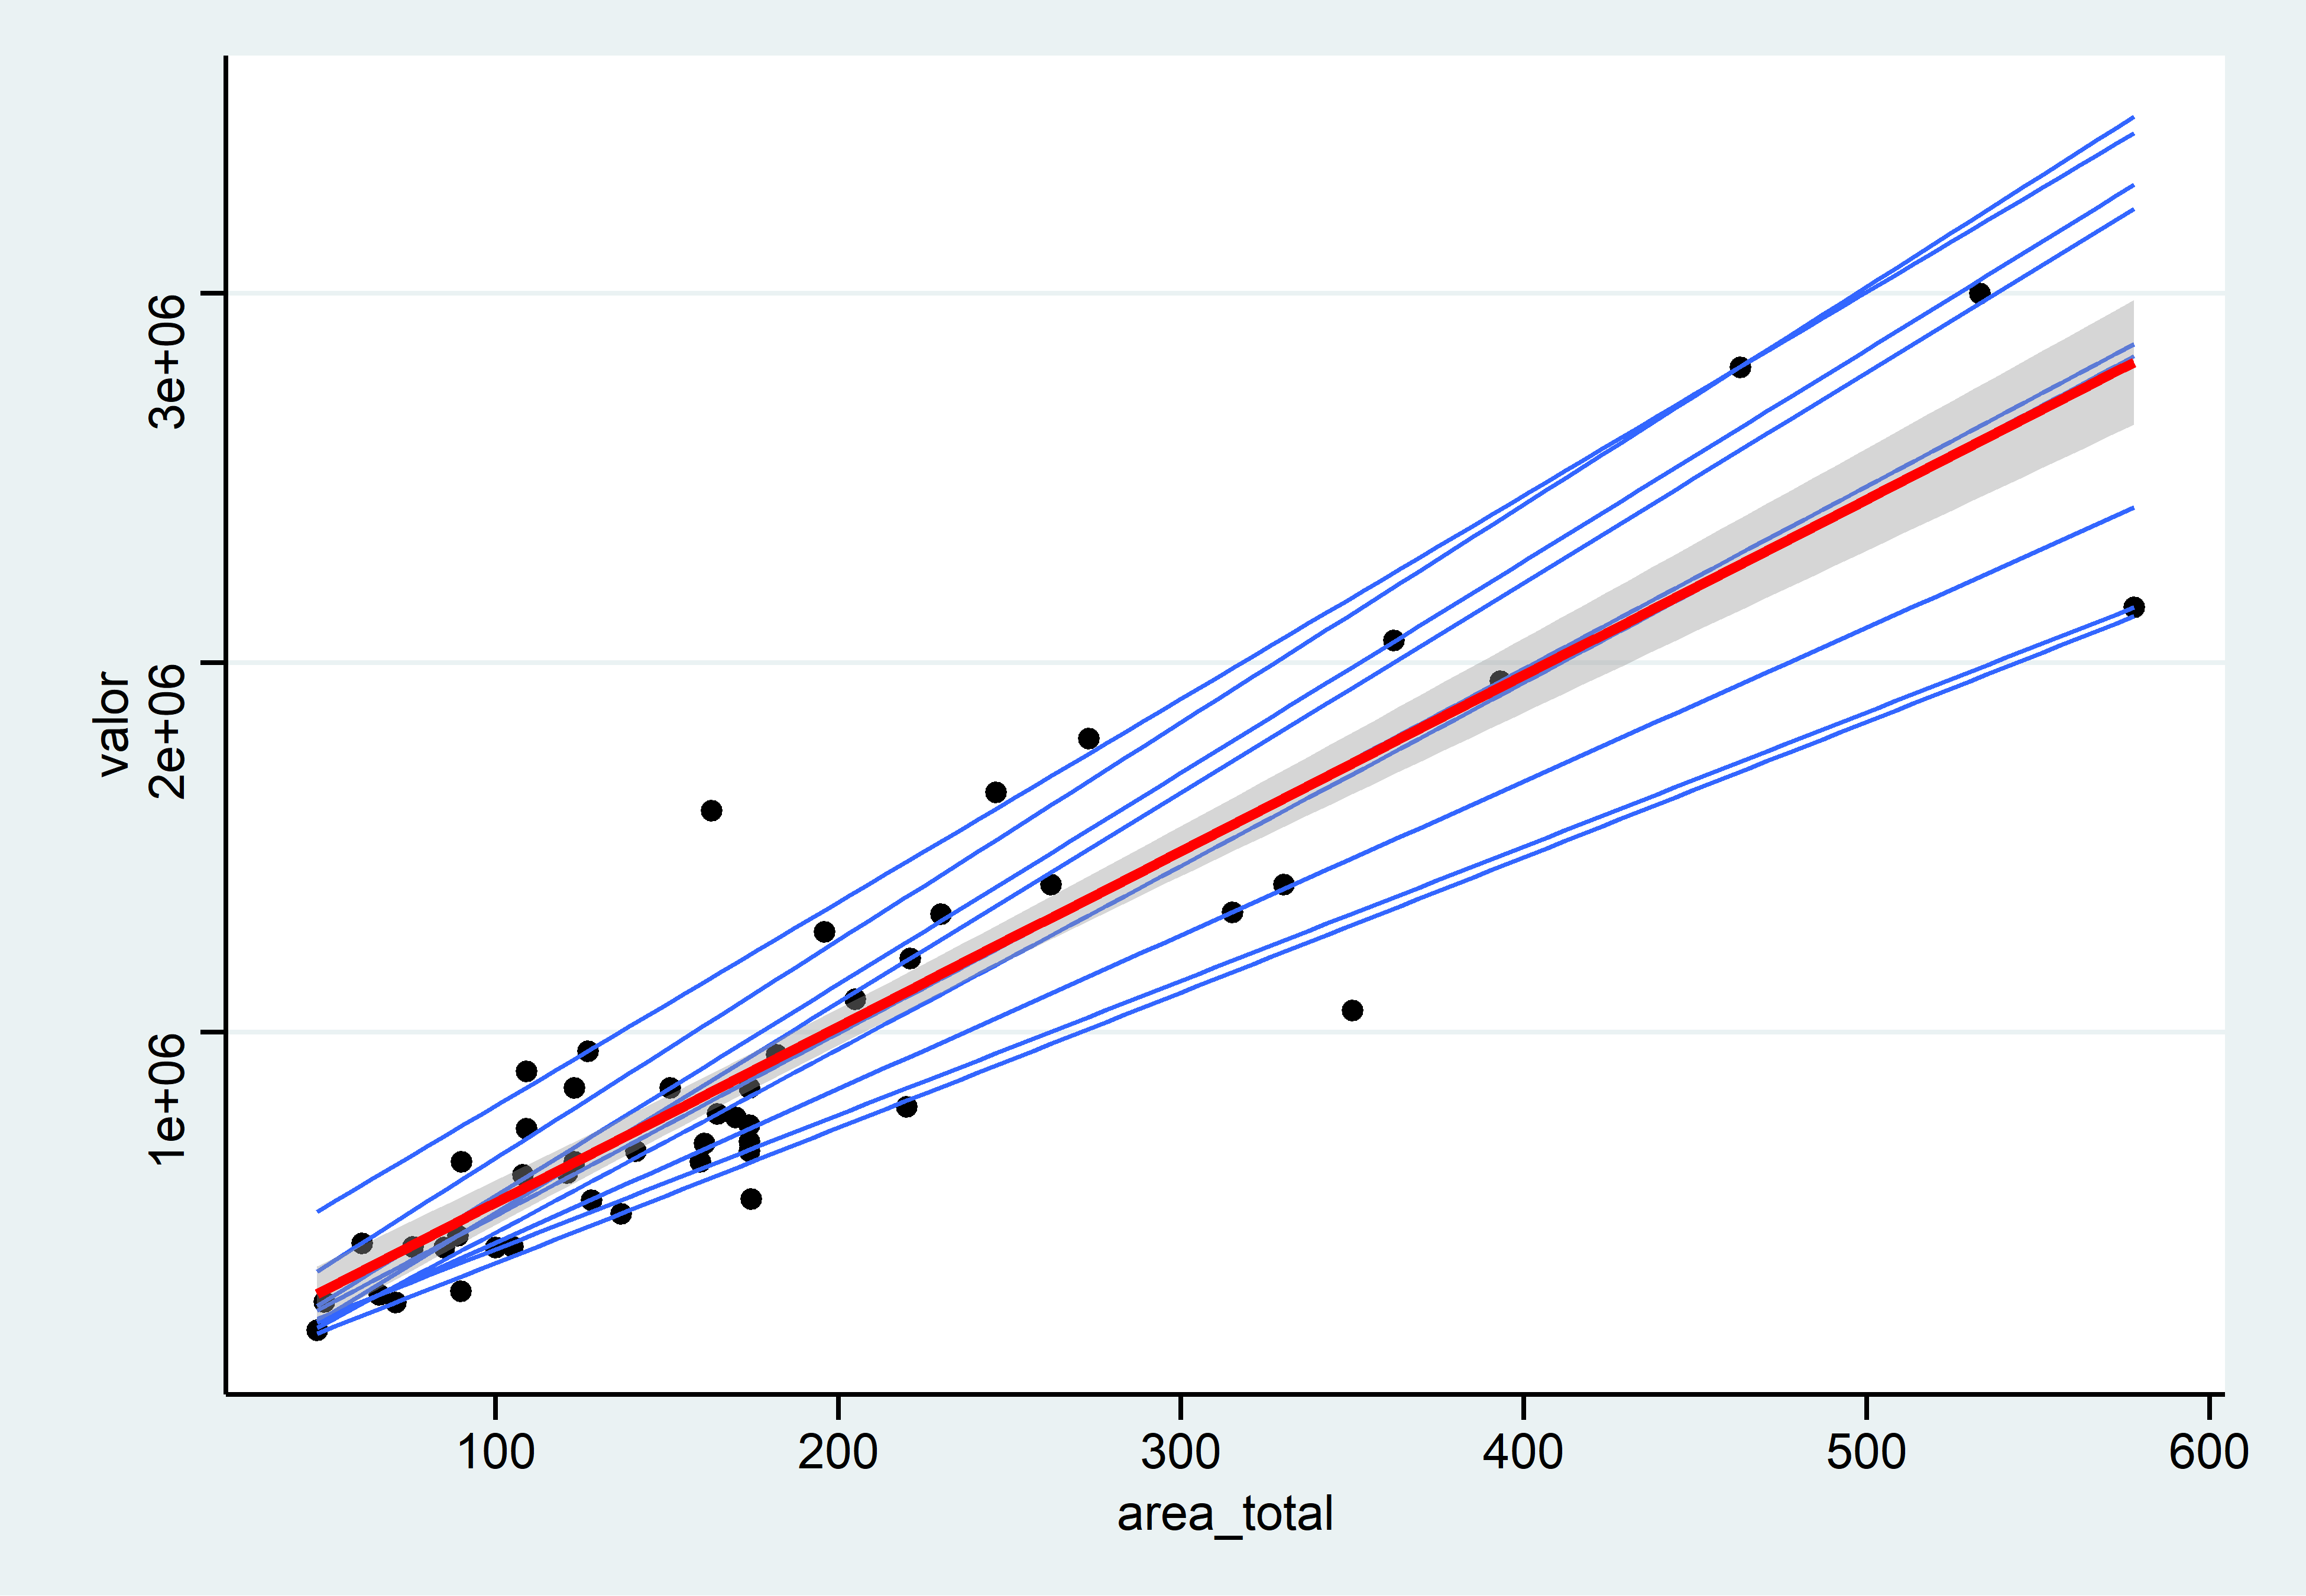
\includegraphics[width=0.7\linewidth]{images/qr1-1} 

}

\caption{Regressão Linear e Quantílica para dados heteroscedásticos.}\label{fig:qr1}
\end{figure}

Assim como na regressão linear, uma conveniente transformação das
variáveis pode ser aplicada para a obtenção da homoscedasticidade. Isto
pode ser visto na figura \ref{fig:qr2}, onde as retas para os diferentes
quantis obtidas pela regressão quantílica agora são praticamente
paralelas entre si, indicando que a heteroscedasticidade foi removida.

\begin{figure}[H]

{\centering 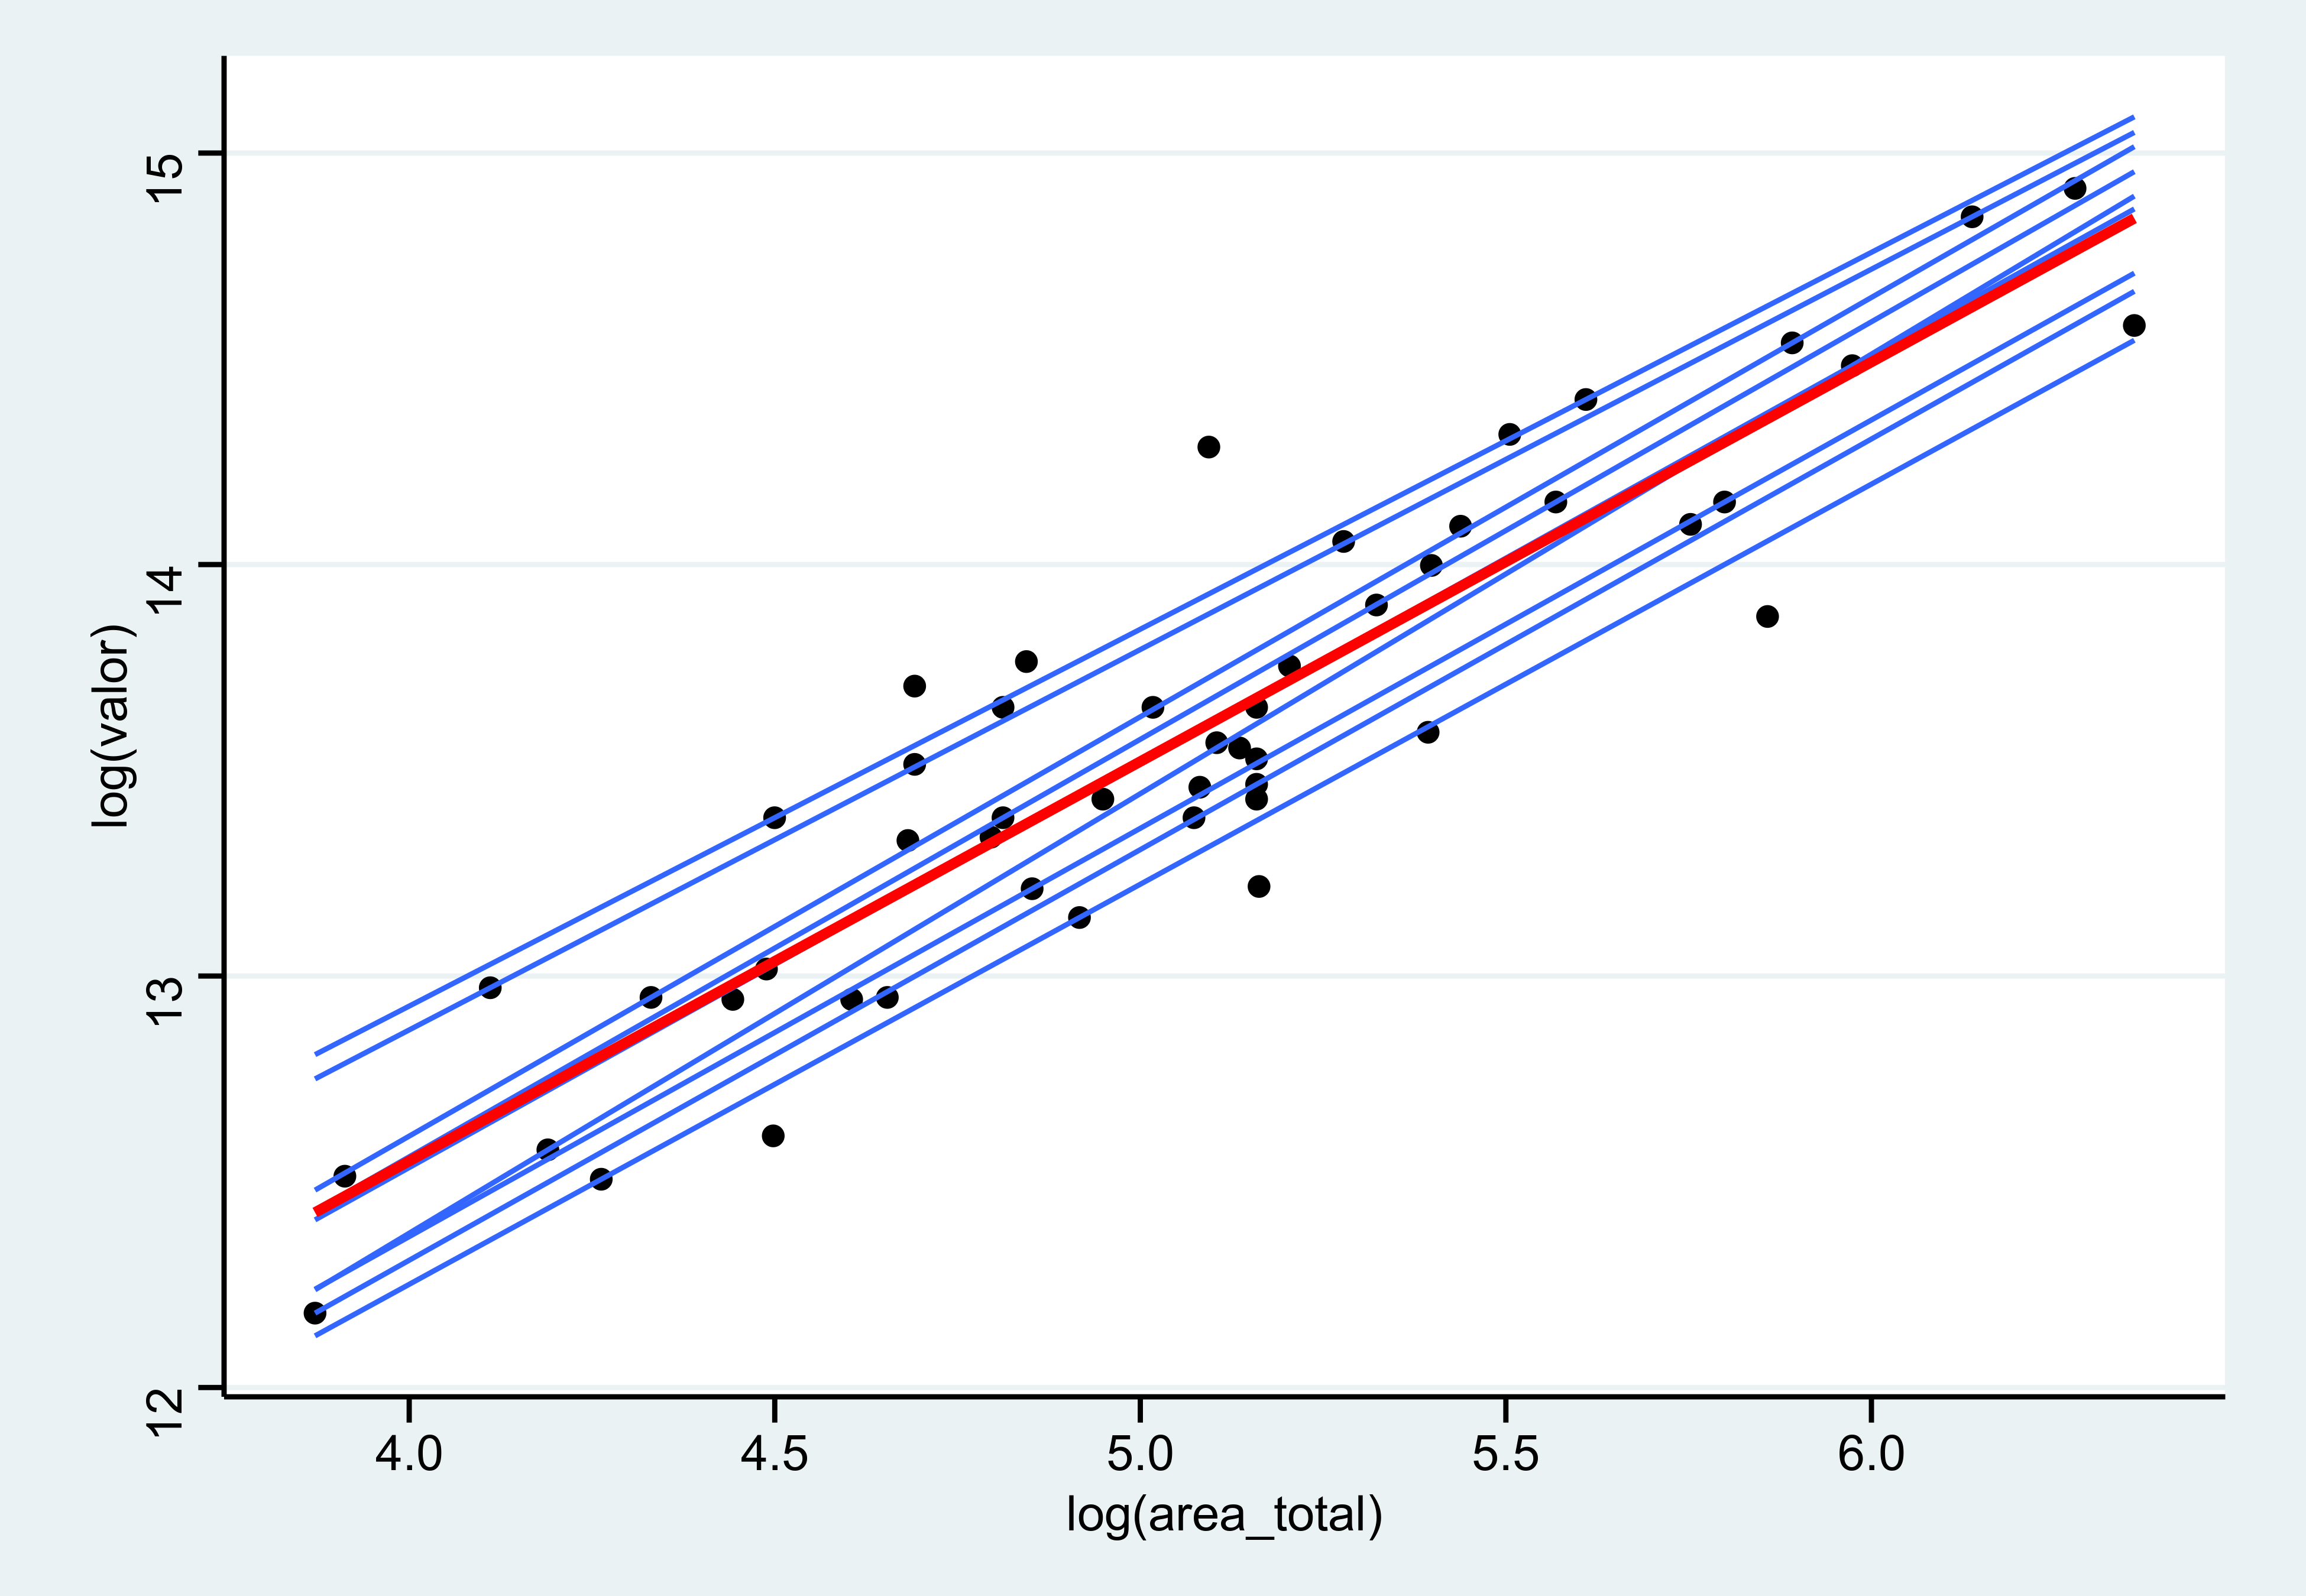
\includegraphics[width=0.7\linewidth]{images/qr2-1} 

}

\caption{Regressão Linear e Quantílica com dados transformados.}\label{fig:qr2}
\end{figure}

Os coeficientes das retas de regressão quantílica podem ser plotados
como na figura \ref{fig:coef1}. Nesta figura, a reta cheia vermelha
representa o coeficiente do modelo de regressão linear, enquanto a reta
preta pontilhada representa os vários coeficientes da regressão
quantílica. As retas vermelhas tracejadas representam o intervalo de
confiança de estimação do coeficiente de regressão linear. A área
sombreada em cinza representa os intervalos de confiança para os
coeficientes da regressão quantílica. Deve-se notar que, entre os
quantis aproximados de 0,3 e 0,55, os coeficientes da regressão
quantílica não são significamente diferentes, estatísticamente, do
coeficiente da regreessão linear.

\begin{figure}[H]

{\centering 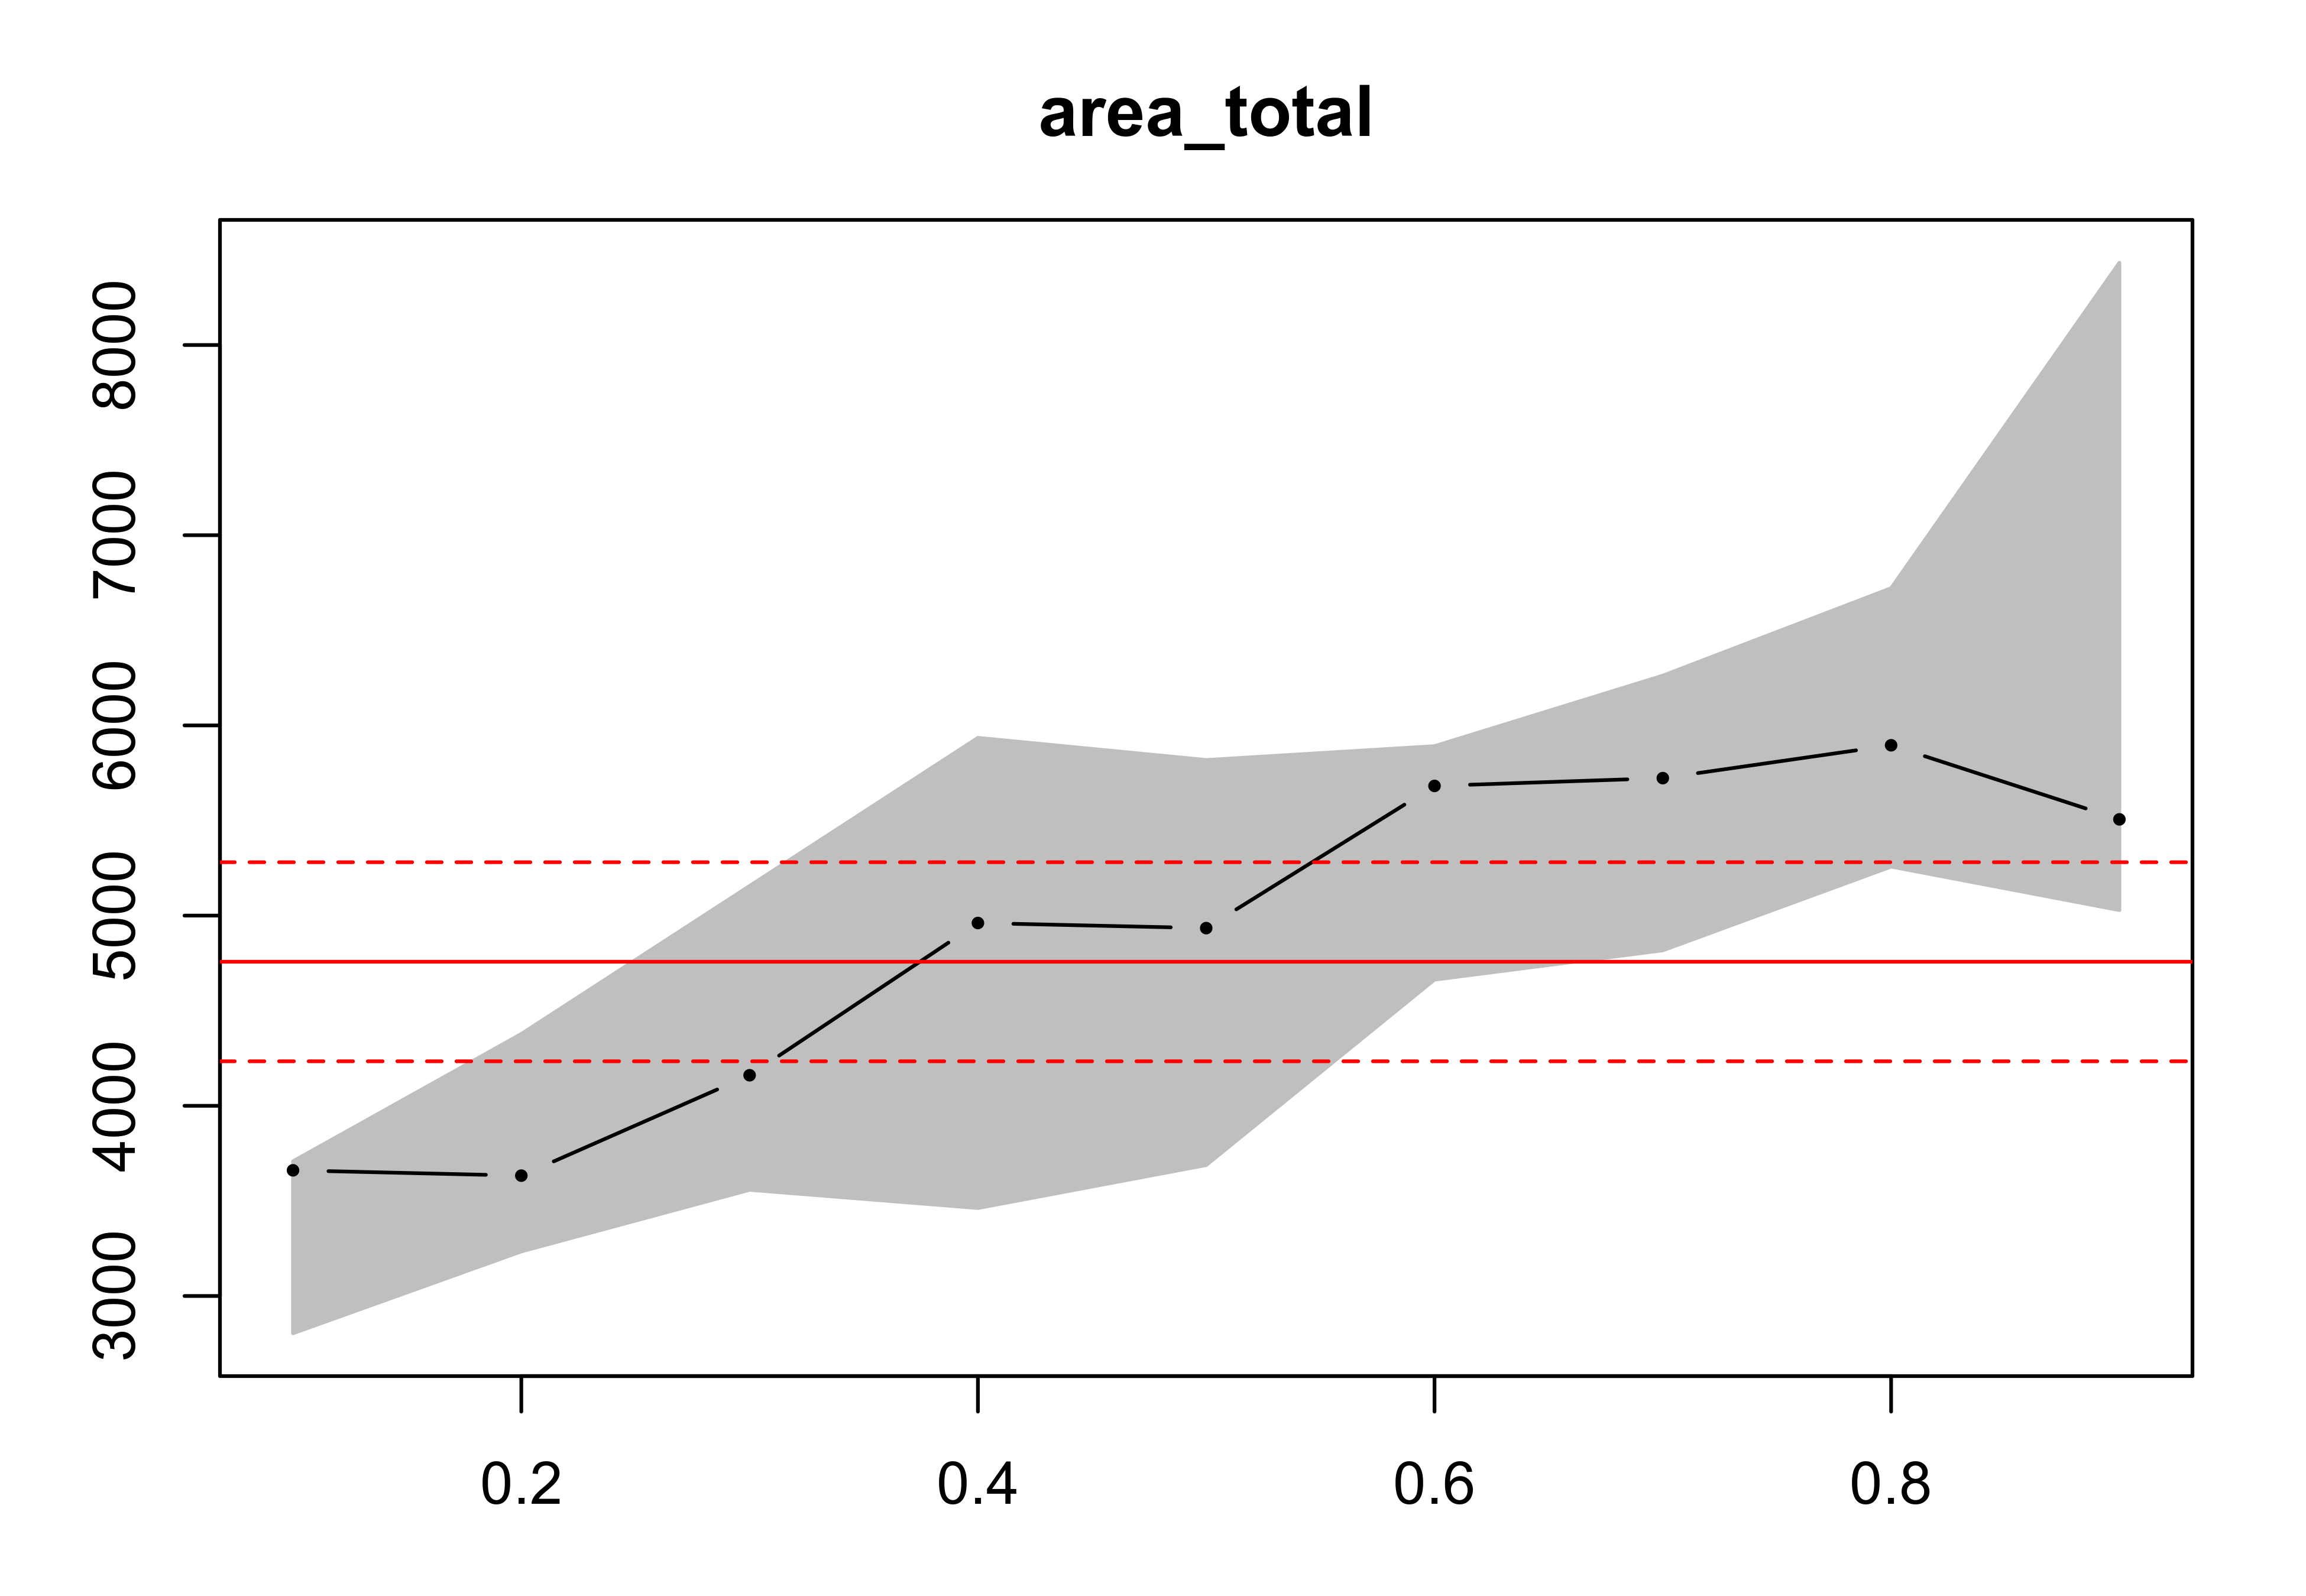
\includegraphics[width=0.7\linewidth]{images/coef1-1} 

}

\caption{Variação dos coeficientes de regressão quantílica (variáveis originais).}\label{fig:coef1}
\end{figure}

Já para os dados transformados, pode-se notar na figura \ref{fig:coef2}
que para todos os quantis, os coeficientes da regressão quantílica não
podem ser considerados estatisticamente diferentes do coeficiente da
regressão linear. Também se pode notar nesta figura como o estimador de
regressão linear, para uma variável normalmente distribuída e na
ausência de heteroscedasticidade, é mais eficiente do que o estimador da
regressão quantílica, como a teoria já prevê (ver MATLOFF
(\protect\hyperlink{ref-matloff2017}{2017}), 238).

(Zilli, não sei se tu pesquisou isso na revisão bibliográfica, mas acho
que se não, era bom colocar! Colocar algo do tipo: as vantagens e
desvantagens da regressão quantílica. Apesar da regressão quantílica ser
robusta à presença de \emph{outliers}, ela é menos eficiente do que a
regressao linear, caso a distribuição da variável estudada seja normal,
claro.)

\begin{figure}[H]

{\centering 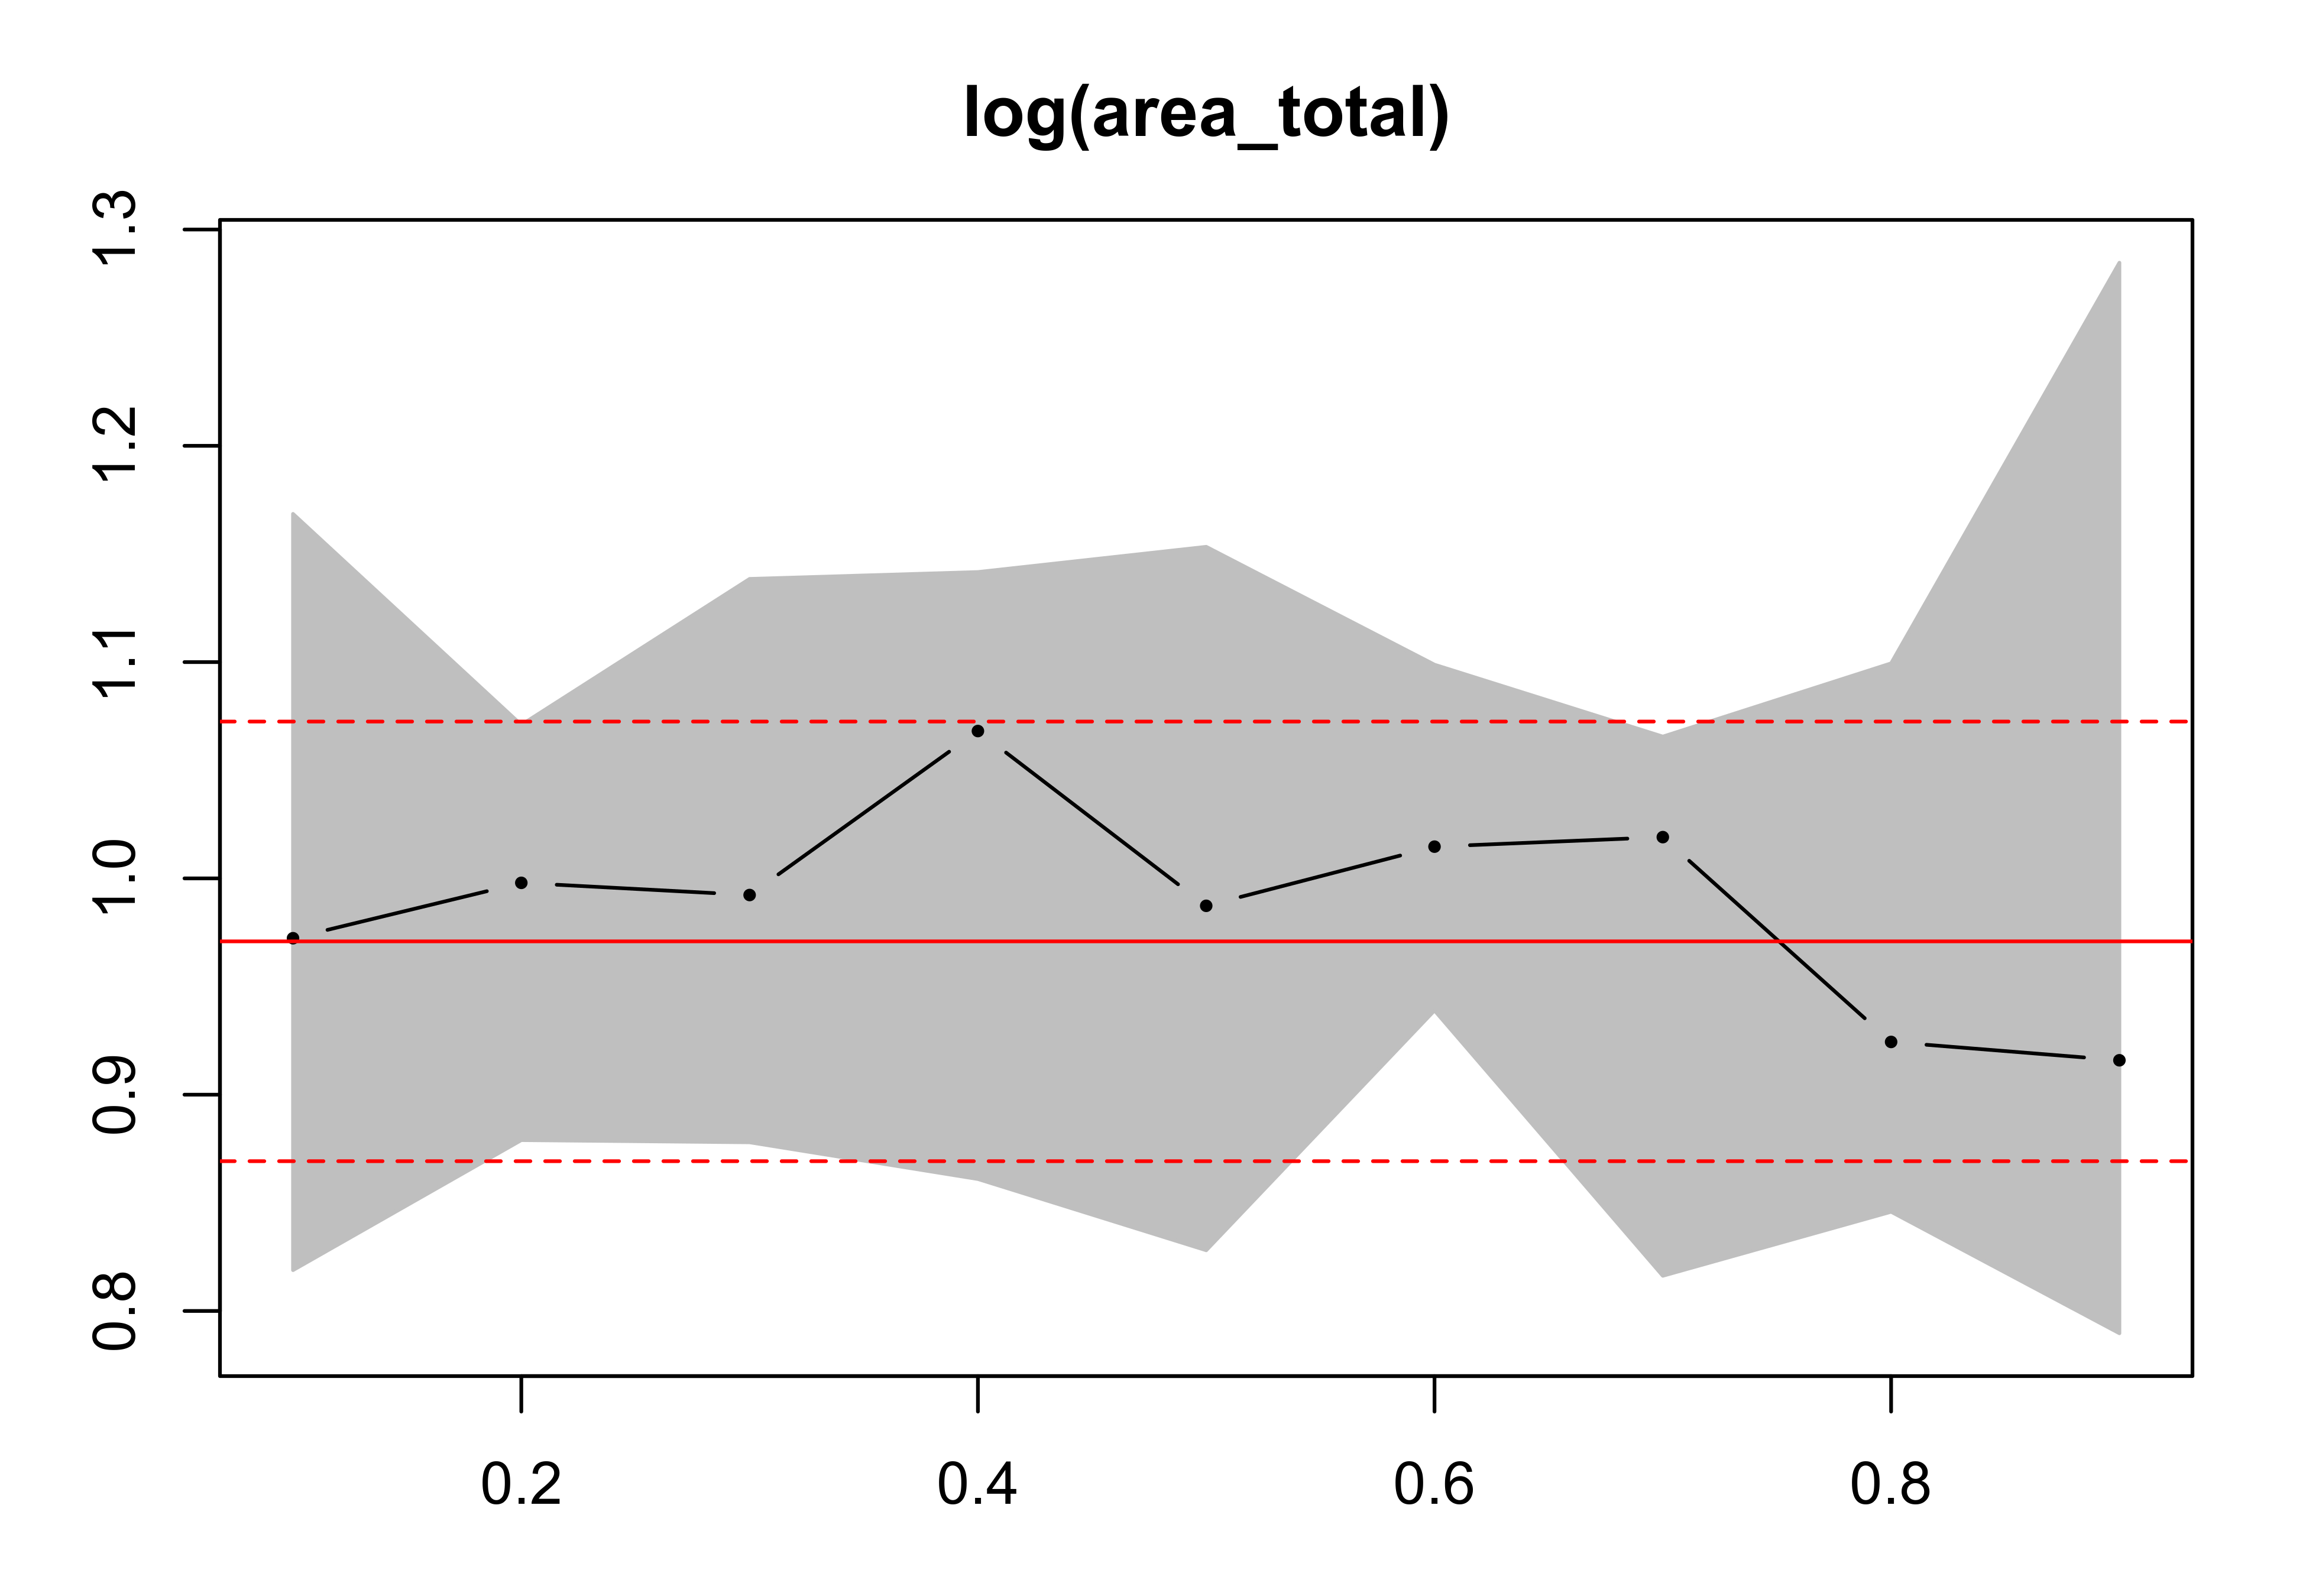
\includegraphics[width=0.7\linewidth]{images/coef2-1} 

}

\caption{Variação dos coeficientes de regressão quantílica (variáveis transformadas).}\label{fig:coef2}
\end{figure}

\hypertarget{analise-multivariada}{%
\subsection{Análise Multivariada}\label{analise-multivariada}}

Para os dados obtidos de Hochheim
(\protect\hyperlink{ref-hochheim}{2015}, pp. 22--23) foram ajustados
dois modelos, um de regressão linear, com os dados saneados, e outro de
regressão quantílica, utilizando-se a totalidade dos dados, para os
quantis 0,1; 0,2; 0,3; 0,4; 0,5; 0,6; 0,7; 0,8 e 0,9.

Na figura \ref{fig:coefs} podem ser vistos os valores dos coeficientes
de cada variável para os diferentes quantis. Pode-se perceber, mais uma
vez, que o valor dos coeficientes da regressão quantílica não diferem
significantemente dos coeficientes da regressão linear (exceção para
alguns quantis superiores nas variáveis \texttt{area\_total} e
\texttt{padrao}).

\begin{figure}[H]

{\centering 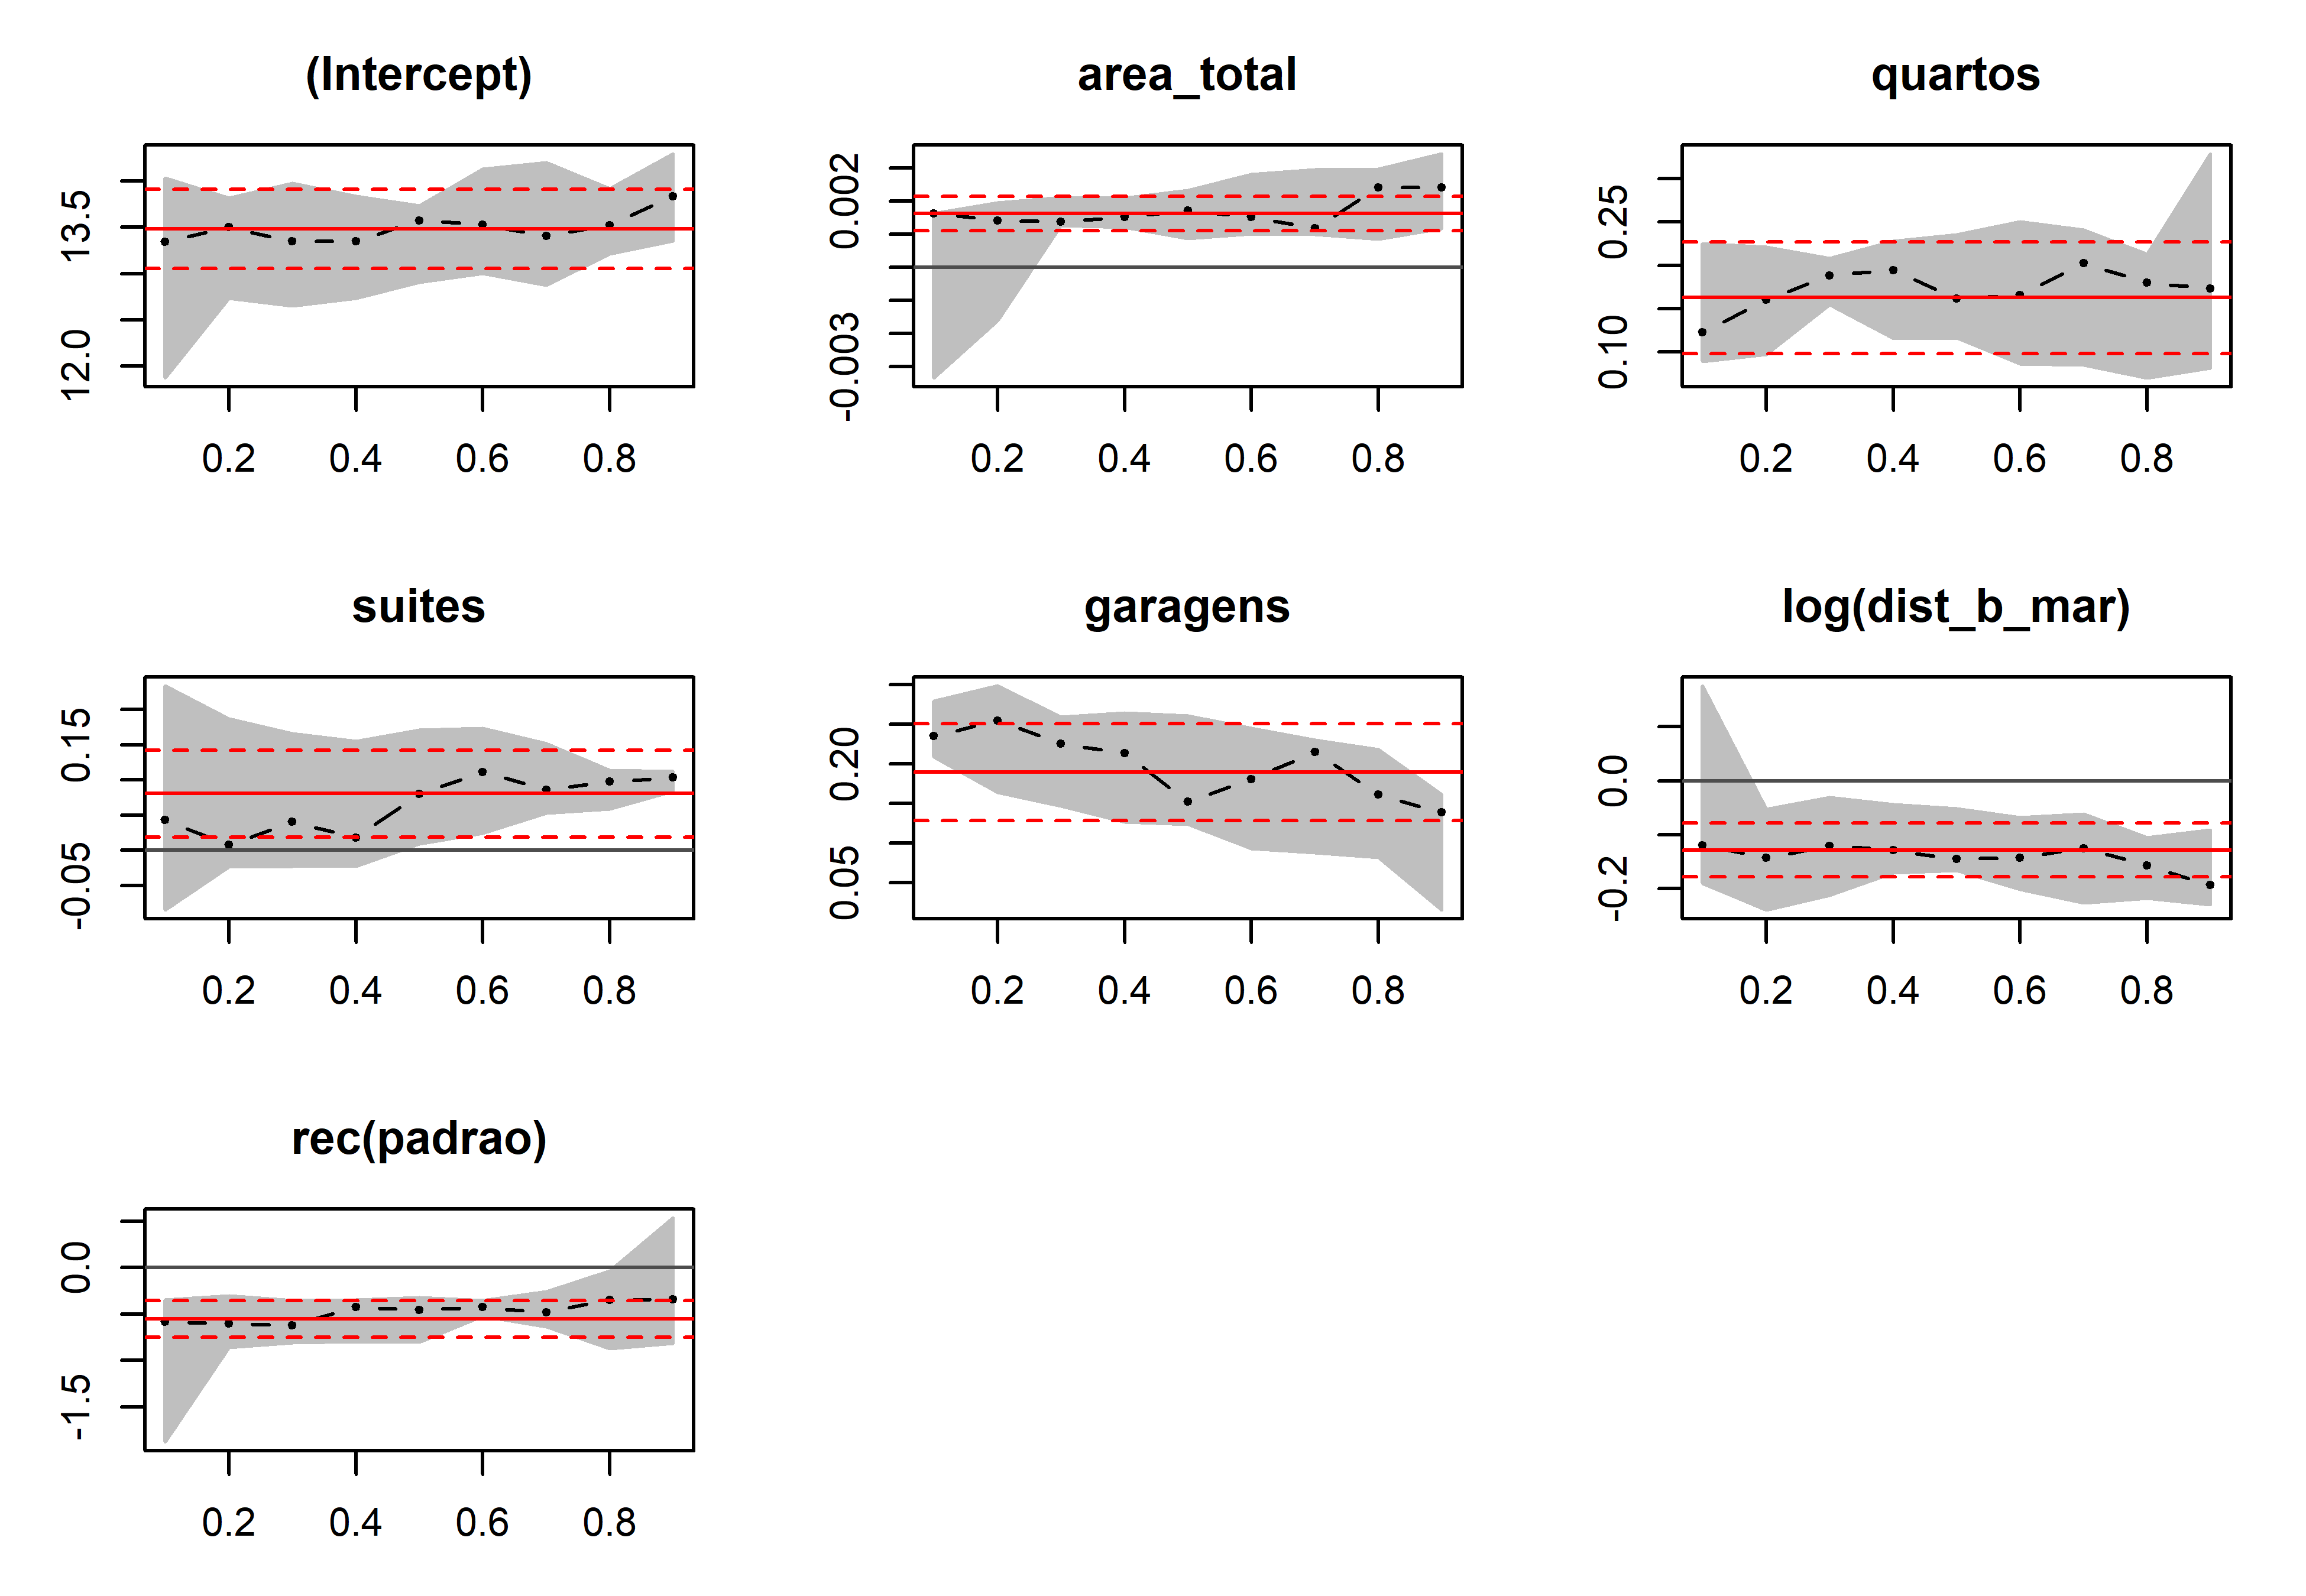
\includegraphics[width=1\linewidth]{images/coefs-1} 

}

\caption{Coeficientes de regressão linear e quantílica. Análise multivariada.}\label{fig:coefs}
\end{figure}

Na tabela \ref{tab:fits} podem ser vistos os coeficientes e estatísticas
básicas dos modelos de regressão linear e de regressão à mediana
(quantil 0,5).

\begin{table}[!htbp] \centering 
  \caption{Comparação entre os modelos de regressão linear e regressão à mediana.} 
  \label{tab:fits} 
\begin{tabular}{@{\extracolsep{5pt}}lcc} 
\\[-1.8ex]\hline 
\hline \\[-1.8ex] 
 & \multicolumn{2}{c}{\textit{Dependent variable:}} \\ 
\cline{2-3} 
\\[-1.8ex] & \multicolumn{2}{c}{log(valor)} \\ 
\\[-1.8ex] & \textit{OLS} & \textit{quantile} \\ 
 & \textit{} & \textit{regression} \\ 
\\[-1.8ex] & (1) & (2)\\ 
\hline \\[-1.8ex] 
 area\_total & 0.001 & 0.002 \\ 
  & (0.001, 0.002) & (0.001, 0.003) \\ 
  & t = 5.113 & t = 2.300 \\ 
  & p = 0.00001$^{***}$ & p = 0.027$^{**}$ \\ 
  & & \\ 
 quartos & 0.164 & 0.162 \\ 
  & (0.118, 0.209) & (0.107, 0.217) \\ 
  & t = 4.626 & t = 3.788 \\ 
  & p = 0.00004$^{***}$ & p = 0.0005$^{***}$ \\ 
  & & \\ 
 suites & 0.061 & 0.080 \\ 
  & (0.018, 0.104) & (0.020, 0.139) \\ 
  & t = 1.810 & t = 1.712 \\ 
  & p = 0.078$^{*}$ & p = 0.095$^{*}$ \\ 
  & & \\ 
 garagens & 0.209 & 0.152 \\ 
  & (0.166, 0.252) & (0.075, 0.230) \\ 
  & t = 6.247 & t = 2.520 \\ 
  & p = 0.00000$^{***}$ & p = 0.016$^{**}$ \\ 
  & & \\ 
 log(dist\_b\_mar) & $-$0.141 & $-$0.146 \\ 
  & ($-$0.176, $-$0.106) & ($-$0.210, $-$0.081) \\ 
  & t = $-$5.174 & t = $-$2.904 \\ 
  & p = 0.00001$^{***}$ & p = 0.006$^{***}$ \\ 
  & & \\ 
 rec(padrao) & $-$0.563 & $-$0.459 \\ 
  & ($-$0.697, $-$0.428) & ($-$0.650, $-$0.267) \\ 
  & t = $-$5.360 & t = $-$3.070 \\ 
  & p = 0.00001$^{***}$ & p = 0.004$^{***}$ \\ 
  & & \\ 
 Constant & 13.564 & 13.574 \\ 
  & (13.268, 13.859) & (13.100, 14.047) \\ 
  & t = 58.847 & t = 36.732 \\ 
  & p = 0.000$^{***}$ & p = 0.000$^{***}$ \\ 
  & & \\ 
\hline \\[-1.8ex] 
Observations & 48 & 50 \\ 
R$^{2}$ & 0.956 &  \\ 
Adjusted R$^{2}$ & 0.950 &  \\ 
Residual Std. Error & 0.136 (df = 41) &  \\ 
F Statistic & 148.921$^{***}$ (df = 6; 41) &  \\ 
\hline 
\hline \\[-1.8ex] 
\textit{Note:}  & \multicolumn{2}{r}{$^{*}$p$<$0.1; $^{**}$p$<$0.05; $^{***}$p$<$0.01} \\ 
\end{tabular} 
\end{table}

\hypertarget{estimativas}{%
\subsubsection{Estimativas}\label{estimativas}}

É interessante comparar as estimativas obtidas com os modelos de
regressão linear, com dados saneados, e o modelo de regressão à mediana,
com a totalidade dos dados. Por um lado, o modelo de regressão linear
tende a ser mais preciso para a estimação da média, como prevê a teoria.
Por outro lado, com mais dados, o modelo de regressão à mediana pode
tornar-se mais eficiente.

Deve-se levar em conta que as estimativas com o modelo de regressão
linear aqui apresentadas são para a mediana da distribuição lognormal.

Pelo modelo de regressão linear, o valor da estimativa central
encontrado foi de R\$961.660,64, com intervalo de confiança entre R\$
924.768,13 e R\$ 1.000.024,94. A amplitude do intervalo de confiança foi
de 7,83\%.

Já pelo modelo de regressão quantílica, o valor da estimativa central
encontrado foi de R\$946.467,87, com intervalo de confiança entre R\$
886.472,34 e R\$ 1.010.523,85. A amplitude do intervalo de confiança foi
de 13,10\%.

O modelo de regressão linear mostrou-se, portanto, mais eficiente do que
o modelo de regressão a mediana, apesar no menor número de dados.

Os limites inferior e superior do intervalo de predição @80\% para o
modelo de regressão linear são, respectivamente: R\$ 802.017,63 e R\$
1.153.080,88.

Para o modelo de regressão quantílica, o intervalo de predição não faz
qualquer sentido. No entanto, é possível estimar os valores diretamente
para os quantis 0,1 e 0,9 da população. Nesta caso, os valores
encontrados foram, respectivamente: R\$ 810.629,32 e R\$ 1.186.954,14.

Podem ainda ser calculados os intervalos de confiança @80\% para as
estimativas dos quantis 0,1 e 0,9.

Os limites inferior e superior do IC para o quantil 0,1 são,
respectivamente: R\$ 781.253,06 e R\$ 841.110,17.

Os limites inferior e superior do IC para o quantil 0,9 são,
respectivamente: R\$ 1.116.547,53 e R\$ 1.261.800,41.

\hypertarget{referencias}{%
\section*{Referências}\label{referencias}}
\addcontentsline{toc}{section}{Referências}

\hypertarget{refs}{}
\leavevmode\hypertarget{ref-hochheim}{}%
HOCHHEIM, N. \textbf{Engenharia de avaliações - módulo básico}.
Florianópolis: IBAPE - SC, 2015.

\leavevmode\hypertarget{ref-matloff2017}{}%
MATLOFF, N. \textbf{From linear models to machine learning: Regression
and classification, with R examples}. Chapman \& Hall, 2017.


\end{document}
